\documentclass[conference]{IEEEtran}
\IEEEoverridecommandlockouts
% The preceding line is only needed to identify funding in the first footnote. If that is unneeded, please comment it out.
\usepackage{cite}
\usepackage{amsmath,amssymb,amsfonts}
\usepackage{algorithmic}
\usepackage{graphicx}
\usepackage{textcomp}
\usepackage{xcolor}
% \usepackage[utf8]{inputenc}
\usepackage{url}
% \usepackage{natbib}
\usepackage{booktabs} 
\usepackage{pgfplots} % For plotting
\pgfplotsset{compat=1.17}
\usepackage{tabularx}
\usepackage{array}

\def\BibTeX{{\rm B\kern-.05em{\sc i\kern-.025em b}\kern-.08em
    T\kern-.1667em\lower.7ex\hbox{E}\kern-.125emX}}
\begin{document}

\title{Deep Learning Enhanced Stereo Vision for LiDAR Emulation in Precise Robotic Arm Manipulation}

% \author{\IEEEauthorblockN{Nazib Abrar}
% \IEEEauthorblockA{\textit{dept. of Mechatronics Engineering} \\
% \textit{Rajshahi University of Engineering \& Technology}\\
% Rajshahi, Bangladesh \\
% abrarnazib@gmail.com}
% \and
% \IEEEauthorblockN{Sarafat Hussain Abhi}
% \IEEEauthorblockA{\textit{dept. of Mechatronics Engineering} \\
% \textit{Rajshahi University of Engineering \& Technology}\\
% Rajshahi, Bangladesh \\
% abhi@mte.ruet.ac.bd}
% }

\author{
\IEEEauthorblockN{\vphantom{A}} % Create an invisible box the height 
\IEEEauthorblockA{\vspace{3\baselineskip}} % Add vertical space
\and
\IEEEauthorblockN{\vphantom{A}}
\IEEEauthorblockA{\vspace{3\baselineskip}}
}

\maketitle

\begin{abstract}
This paper presents a deep learning-augmented stereo vision system designed to emulate LiDAR-grade depth maps for precise robotic arm manipulation in static environments. We developed a prototype integrating stereo cameras with a Time-of-Flight (ToF) camera for ground-truth depth data and a custom 4-DOF robotic arm. A Pyramid Stereo Matching Network (PSMNet) was trained to refine stereo-derived point clouds by minimizing discrepancies with ToF data. In spite of difficulties from lighting variability and a limited training dataset, the custom-trained network significantly improved depth map accuracy, achieving a 27\% reduction in End-Point Error (EPE) compared to a traditional SGBM baseline. These findings demonstrate that while deep learning-augmented stereo vision can approximate LiDAR-level mapping, its reliability is contingent on domain-specific training and controlled environmental conditions, positioning it as a viable, cost-effective solution for depth estimation in robotics.
\end{abstract}

\begin{IEEEkeywords}
stereo vision, deep learning, LiDAR emulation, robotic arm, depth estimation, PSMNet, camera calibration, SGBM
\end{IEEEkeywords}

\section{Introduction}
 Traditional methods for acquiring high-fidelity depth information frequently rely on Light Detection and Ranging (LiDAR) systems, recognized for their precision and reliability \cite{wang2023multi}. However, their high cost and complexity limit extensive utilization, particularly in static environments where cost-effective solutions are desirable \cite{son2019lightweight}.

Stereo vision systems present a viable and more economical alternative by reconstructing depth from visual discrepancies between images. While affordable, stereo vision encounters difficulties in depth accuracy, especially under varying lighting conditions and due to complex calibration requirements \cite{zhou2006high}. Recent progress in computer vision, particularly with deep learning, have profoundly influenced depth estimation \cite{xu2025towards}. The evolution from traditional geometric methods to deep learning approaches \cite{rohan2025systematic} indicates a trend towards data-driven methodologies to overcome inherent limitations. This research addresses this gap by investigating LiDAR emulation through an enhanced stereo vision system augmented with deep learning.

The primary objective is to achieve depth estimation accuracy comparable to LiDAR to facilitate precise robotic arm manipulation without high costs. This is realized by training Deep Neural Networks (DNNs) on datasets derived from Time-of-Flight (ToF) cameras, which serve as a reliable source of ground truth depth data, to correct and refine stereo vision depth maps \cite{agresti2019stereo}.

The key contributions of this study include:
\begin{itemize}
    \item Development of a prototype system integrating a custom-built four-degree-of-freedom (4-DOF) robotic arm with a stereo camera setup and a Time-of-Flight (ToF) camera.
    \item Implementation of camera calibration and stereo rectification.
    \item Application of the Semi-Global Block Matching (SGBM) algorithm to establish a robust baseline for stereo depth estimation.
    \item Enhancement of stereo depth maps via a comparative deep learning analysis, evaluating the performance of pre-trained PSMNet models against a network custom-trained on our system's domain-specific ground truth data.
    \item Thorough examination of the system's effectiveness and limitations in achieving LiDAR-grade depth emulation.
\end{itemize}
This research frames the problem as an essential need for precise yet affordable depth sensing in robotics, positioning the deep learning-enhanced stereo vision as a viable solution.

\section{Related Work}
The field of depth estimation has experienced substantial developments, particularly with the integration of deep learning techniques, which have addressed many traditional challenges associated with stereo matching. This section reviews recent contributions, contextualizing the presented approach within the broader academic landscape.

\subsection{Deep Learning Advancements in Stereo Matching}
Recent research has focused on enhancing stereo matching through novel deep learning architectures and training paradigms. Wen et al. \cite{wen2025foundationstereo} introduced FoundationStereo, a zero-shot stereo matching model that leverages large-scale synthetic datasets, demonstrating robust generalization.

Further developments integrate monocular depth cues into stereo frameworks; models like DEFOM-Stereo \cite{jiang2025defom} and MonSter \cite{cheng2025monster} leverage this hybrid approach to improve accuracy in challenging conditions such as occlusions and textureless regions.

Addressing the scarcity of real-world annotated stereo data, Wang et al. \cite{wang2025stereogen} developed StereoGen, a novel pipeline capable of generating high-quality stereo images from a single input using deep learning. This method synthesizes corresponding right images, enabling impressive generalization across various environments.

Comprehensive reviews, such as that by Rohan et al. \cite{rohan2025systematic}, provide a systematic overview of deep learning-based depth estimation. These reviews highlight the evolution of techniques from monocular to stereo and multi-view approaches, emphasizing the critical role of large datasets and advanced neural architectures in improving depth estimation accuracy and generalization capabilities. 

Such analyses underscore the ongoing challenges, including the need for extensive manual tuning and the difficulty of generalizing models to diverse, unseen scenes. While models pre-trained on large-scale public datasets (e.g., for autonomous driving or synthetic scenes) achieve state-of-the-art performance, their effectiveness can be limited by domain shift when applied to specialized tasks such as indoor robotic manipulation. This progression, coupled with the challenge of domain adaptation, directly informs our selection of a robust architecture like PSMNet and our methodological focus on evaluating the benefits of custom, domain-specific training.

\subsection{Applications of Stereo Vision in Robotics}
Stereo vision is a pivotal tool for various robotic applications, particularly those requiring precise 3D perception. Perezyabov et al. \cite{perezyabov2022depth} demonstrated the utility of stereo cameras for road obstacle detection. Their method combines depth and image data to enhance detection accuracy, addressing the limitations of monocular systems.

In the context of robotic manipulation, depth perception plays a critical role in 3D object localization and interaction \cite{guo2025monocular, li2024virt, correll2024versatile, chen2024bio}. Many studies in this domain focus on 6D pose estimation for grasping, a task that relies heavily on accurate depth sensing \cite{du2021vision}. The integration of advanced vision systems enables robots to perceive and interact with their environment with high precision, moving beyond simple pick-and-place operations to more complex, dexterous manipulations. The literature consistently highlights the critical need for accurate depth perception in robotic manipulation and the growing role of deep learning in enhancing vision systems for this purpose, reinforcing the practical relevance and timeliness of the current research.

% \section{Introduction}
% Accurate depth perception is fundamental for robotic arm manipulation, enabling effective interaction with objects in a workspace \cite{du2021vision, guo2025monocular}. While Light Detection and Ranging (LiDAR) systems offer high-fidelity depth data, their cost and complexity limit adoption in applications like static industrial automation where cost-effective solutions are paramount \cite{wang2023multi, son2019lightweight}. Stereo vision presents an economical alternative by reconstructing depth from binocular parallax but often suffers from lower accuracy due to lighting variability and complex calibration \cite{zhou2006high}.

% Recent advances in deep learning offer a data-driven path to overcome these limitations, significantly improving depth estimation from images \cite{xu2025towards, rohan2025systematic, zhang2025survey}. This research bridges the gap by developing a deep learning-enhanced stereo vision system to emulate LiDAR performance. Our primary objective is to achieve high-accuracy depth maps for precise robotic manipulation by training a Deep Neural Network (DNN) on stereo images, using a co-located Time-of-Flight (ToF) camera for ground-truth depth data \cite{hansard2012time, agresti2019stereo}.

% The key contributions of this work are: 1) the development of an integrated prototype featuring a 4-DOF robotic arm, a stereo camera rig, and a ToF camera for data acquisition; 2) the implementation of a robust calibration pipeline and a traditional Semi-Global Block Matching (SGBM) algorithm to establish a performance baseline; 3) the enhancement of depth estimation using a custom-trained Pyramid Stereo Matching Network (PSMNet), which leverages ToF data as ground truth; and 4) a comprehensive analysis of the system's effectiveness and limitations in achieving LiDAR-grade depth emulation. This work positions our approach as a viable solution for affordable, high-precision depth sensing in robotics.

% \section{Related Work}
% The field of depth estimation has advanced significantly with the integration of deep learning, addressing many traditional stereo matching challenges. This section reviews key contributions, contextualizing our approach within the academic landscape.

% \subsection{Deep Learning Advancements in Stereo Matching}
% Recent research has focused on novel deep learning architectures to enhance stereo matching. Wen et al. introduced FoundationStereo, a zero-shot model that demonstrates robust generalization by leveraging large-scale synthetic datasets \cite{wen2025foundationstereo}. Other advancements integrate monocular depth cues into stereo frameworks; models like DEFOM-Stereo \cite{jiang2025defom} and MonSter \cite{cheng2025monster} use this hybrid approach to improve accuracy in occluded or textureless regions. To address the scarcity of annotated real-world data, Wang et al. developed StereoGen, a pipeline that generates high-quality stereo pairs from a single image, enabling impressive generalization \cite{wang2025stereogen}.

% Comprehensive surveys, such as that by Rohan et al. \cite{rohan2025systematic}, highlight the evolution from traditional algorithms to advanced neural architectures. They underscore ongoing challenges, including generalization to unseen scenes and the need for extensive tuning. This progression towards models that leverage global context to overcome the inherent limitations of local stereo matching directly informs our selection of PSMNet for enhancing depth estimation.

% \subsection{Applications of Stereo Vision in Robotics}
% Stereo vision is a pivotal sensor for robotic applications requiring 3D perception. For instance, Perezyabov et al. demonstrated its utility for road obstacle detection by fusing depth and image data to improve accuracy over monocular systems \cite{perezyabov2022depth}. In robotic manipulation, accurate depth perception is critical for tasks like 6D object pose estimation and grasping \cite{du2021vision, guo2025monocular, li2024virt, correll2024versatile, chen2024bio}. Advanced vision systems enable robots to perform complex, dexterous manipulations beyond simple pick-and-place operations \cite{yuan2024hierarchical}. The literature consistently highlights the need for precise depth sensing in robotic manipulation and the growing role of deep learning in vision systems, reinforcing the practical relevance of our research.


\section{Methodology}
This section details the experimental setup, calibration procedures, and algorithms used to achieve deep learning-enhanced stereo vision.

\subsection{Hardware Setup}
The hardware consists of a custom robotic arm and an integrated vision system. The manipulation platform is a custom-built 4-DOF robotic arm fabricated from 3D-printed PLA , 
aluminium rods, actuated by NEMA 17 stepper motors with TMC2208 drivers and controlled by an Arduino Uno with a CNC shield.

The vision system integrates a Time-of-Flight (ToF) camera (MaixSense-A075V) for ground-truth depth data \cite{hansard2012time} and two Fantech Luminous C30 cameras for stereo vision. The ToF camera has a depth resolution of 320x240 and an operating range of 0.15 to 1.5 meters. The stereo cameras provide a 2560x1440 resolution. The complete system, including the robotic arm and top-mounted cameras, is assembled within a structured workspace to ensure controlled data collection, as depicted in Figures \ref{fig:robotic_arm}, \ref{fig:cameras}, and \ref{fig:workspace}.

% --- Figures from original Methodology section ---
\begin{figure}[htbp]
\centerline{\includegraphics[width=0.7\columnwidth]{robotic_arm.jpg}}
\caption{Custom-built 4-DOF robotic arm.}
\label{fig:robotic_arm}
\end{figure}

\begin{figure}[htbp]
\centerline{\includegraphics[width=\columnwidth]{camera_setup.png}}
\caption{ToF and Stereo Camera System.}
\label{fig:cameras}
\end{figure}

\begin{figure}[htbp]
\centerline{\includegraphics[width=0.7\columnwidth]{workspace_setup.jpg}}
\caption{Workspace setup for data acquisition and robotic arm operation.}
\label{fig:workspace}
\end{figure}

\subsection{Camera Calibration}
Camera calibration is a foundational step for geometric accuracy in 3D reconstruction \cite{liao2303deep}. The process corrects lens distortions and provides the parameters for aligning stereo images, which is critical for accurate depth estimation.

% \subsubsection{Epipolar Geometry and Rectification}
% Epipolar geometry describes the relationship between two camera views of a 3D scene \cite{xu2013epipolar, hartley2003multiple}. The camera's intrinsic matrix $\mathbf{K}$ defines its internal optical properties:
% $$\mathbf{K} = \begin{pmatrix} f_x & 0 & c_x \\ 0 & f_y & c_y \\ 0 & 0 & 1 \end{pmatrix} \quad (1)$$
% Extrinsic parameters ($\mathbf{R}$, $\mathbf{t}$) describe the camera's orientation and position:
% $$\mathbf{X}_c = \mathbf{R}\mathbf{X}_w + \mathbf{t} \quad (2)$$
% Lens distortions are modeled using radial ($K_1, K_2, K_3$) and tangential ($P_1, P_2$) coefficients:
% $$x'' = x'(1+K_1r^2+K_2r^4+K_3r^6)+2P_1x'y'+P_2(r^2+2x'^2) \quad (3)$$
% $$y'' = y'(1+K_1r^2+K_2r^4+K_3r^6)+P_1(r^2+2y'^2)+2P_2x'y' \quad (4)$$
% where $r^2=x'^2+y'^2$. Since perfect hardware alignment is impractical, stereo rectification computationally transforms the images to align epipolar lines horizontally, simplifying the correspondence search for disparity calculation \cite{zhao2024dive, gong2025rectification}.

\subsubsection{Epipolar Geometry and Rectification}
Epipolar geometry describes the relationship between two camera views of a 3D scene. The camera's intrinsic matrix $\mathbf{K}$, shown in \eqref{eq:intrinsic_matrix}, defines its internal optical properties:
\begin{equation}
    \mathbf{K} = \begin{pmatrix} f_x & 0 & c_x \\ 0 & f_y & c_y \\ 0 & 0 & 1 \end{pmatrix}
    \label{eq:intrinsic_matrix}
\end{equation}
Extrinsic parameters ($\mathbf{R}$, $\mathbf{t}$) describe the camera's orientation and position relative to a world coordinate system, as defined in \eqref{eq:extrinsic_params}:
\begin{equation}
    \mathbf{X}_c = \mathbf{R}\mathbf{X}_w + \mathbf{t}
    \label{eq:extrinsic_params}
\end{equation}
Lens distortions are modeled using radial ($K_1, K_2, K_3$) and tangential ($P_1, P_2$) coefficients. The corrected image coordinates ($x'', y''$) are calculated from the distorted coordinates ($x', y'$) using the model in \eqref{eq:distort_x} and \eqref{eq:distort_y}:
\begin{equation}
    x'' = x'(1+K_1r^2+K_2r^4+K_3r^6)+2P_1x'y'+P_2(r^2+2x'^2)
    \label{eq:distort_x}
\end{equation}
\begin{equation}
    y'' = y'(1+K_1r^2+K_2r^4+K_3r^6)+P_1(r^2+2y'^2)+2P_2x'y'
    \label{eq:distort_y}
\end{equation}
where $r^2=x'^2+y'^2$. Since perfect hardware alignment is impractical, stereo rectification computationally transforms the images to align epipolar lines horizontally, simplifying the correspondence search for disparity calculation.



\subsubsection{Calibration Process and Results}
We performed calibration using a 9x7 checkerboard pattern, capturing images from multiple perspectives to estimate camera parameters with OpenCV \cite{zhang2002flexible, zhang1999flexible}. The derived intrinsic parameters and distortion coefficients are listed in Table \ref{tab1}. The process resulted in a rectification \textbf{RMS error of 1.509}, confirming successful epipolar alignment as shown in the rectified view in Fig. \ref{fig:rectification}.

% \begin{table}[htbp]
% \caption{Fantech Luminous C30 Camera Intrinsic Parameters and Distortion Coefficients}
% \begin{center}
% % Using booktabs for better formatting as requested
% \begin{tabular}{@{}ll@{}}
% \toprule
% \textbf{Parameter} & \textbf{Value} \\
% \midrule
% $f_x$ & 680.9335952 mm \\
% $f_y$ & 681.53275369 mm \\
% $c_x$ & 322.60859724 px \\
% $c_y$ & 257.99884455 px \\
% $K_1$ & -3.84198386 $\times 10^{-1}$ \\
% $K_2$ & 3.37282195 $\times 10^{-1}$ \\
% $K_3$ & 1.72120651 $\times 10^{-3}$ \\
% $P_1$ & -5.48946011 $\times 10^{-4}$ \\
% $P_2$ & -6.45215020 $\times 10^{-1}$ \\
% \bottomrule
% \end{tabular}
% \label{tab1}
% \end{center}
% \end{table}

% Define the new column type. You can place this in your preamble
% or right before the table. It creates a centered, auto-expanding column.
\newcolumntype{Y}{>{\centering\arraybackslash}X}

\begin{table}[htbp]
\caption{Fantech Luminous C30 Camera Intrinsic Parameters and Distortion Coefficients}
\centering % Use \centering for better spacing than the <center> environment

% Increase row height by 50% to give the content "breathing room"
\renewcommand{\arraystretch}{1.5}

% Use tabularx to create a table that spans the full column width.
% The 'Y' columns will be centered and will share the space equally.
% We use booktabs rules for a clean, professional look without vertical lines.
\begin{tabularx}{\columnwidth}{ Y Y }
\toprule
\textbf{Parameter} & \textbf{Value} \\
\midrule
$f_x$ & 680.9335952 mm \\
$f_y$ & 681.53275369 mm \\
$c_x$ & 322.60859724 px \\
$c_y$ & 257.99884455 px \\
$K_1$ & -3.84198386 $\times 10^{-1}$ \\
$K_2$ & 3.37282195 $\times 10^{-1}$ \\
$K_3$ & 1.72120651 $\times 10^{-3}$ \\
$P_1$ & -5.48946011 $\times 10^{-4}$ \\
$P_2$ & -6.45215020 $\times 10^{-1}$ \\
\bottomrule
\end{tabularx}
\label{tab1}
\end{table}

\begin{figure}[htbp]
\centerline{\includegraphics[width=\columnwidth]{rectified_camera_view.png}}
\caption{Rectified camera view demonstrating epipolar alignment.}
\label{fig:rectification}
\end{figure}

% \subsection{Data Acquisition}
% The data acquisition involved capturing synchronized stereo image pairs ($I_L, I_R$) and ToF depth maps across various scenes. Disparity $d(x, y)$ is the horizontal shift between corresponding points:
% $$d(x, y) = x_L - x_R \quad (5)$$
% Depth $Z$ is then estimated via triangulation:
% $$Z = \frac{f \cdot B}{d(x,y)} \quad (6)$$
% where $f$ is focal length and $B$ is the baseline (84.85mm).

\subsection{Data Acquisition}
The data acquisition involved capturing synchronized stereo image pairs ($I_L, I_R$) and ToF depth maps across various scenes. Disparity $d(x, y)$, which represents the horizontal shift between corresponding points in the stereo pair, is defined in \eqref{eq:disparity}:
\begin{equation}
    d(x, y) = x_L - x_R
    \label{eq:disparity}
\end{equation}
Depth ($Z$) is then estimated from disparity via triangulation, following the fundamental stereo vision formula shown in \eqref{eq:depth_triangulation}:
\begin{equation}
    Z = \frac{f \cdot B}{d(x,y)}
    \label{eq:depth_triangulation}
\end{equation}
where $f$ is the focal length and $B$ is the baseline distance between the stereo cameras (84.85mm in our setup).

\subsection{Depth Estimation (Traditional SGBM)}
A baseline for depth estimation was established using the Semi-Global Block Matching (SGBM) algorithm \cite{hirschmuller2007stereo, hernandez2016embedded}, chosen for its balance of accuracy and computational efficiency. The algorithm was configured with the empirically optimized parameters shown in Table \ref{tab2}. The SGBM method produced reliable depth maps in well-textured regions but struggled with noise in low-texture areas (Fig. \ref{fig:sgbm_depth}).

% \begin{table}[htbp]
% \caption{SGBM Algorithm Optimized Parameters}
% \begin{center}
% % Using booktabs for better formatting as requested
% \begin{tabular}{@{}ll@{}}
% \toprule
% \textbf{Parameter} & \textbf{Value}  \\
% \midrule
% Block Size & 7 pixels  \\
% Disparity Range & 128 levels \\
% Minimum Disparity & 5  \\
% P1 Penalty & 8 * 3 * 7$^2$  \\
% P2 Penalty & 32 * 3 * 7$^2$  \\
% Uniqueness Ratio & 15  \\
% Speckle Window Size & 100  \\
% Speckle Range & 2  \\
% Pre-Filter Cap & 63 \\
% \bottomrule
% \end{tabular}
% \label{tab2}
% \end{center}
% \end{table}

% You should have this defined in your preamble from the previous table:
% \newcolumntype{Y}{>{\centering\arraybackslash}X}

\begin{table}[htbp]
\caption{SGBM Algorithm Optimized Parameters}
\centering % Use \centering for better spacing

% Increase row height for better readability
\renewcommand{\arraystretch}{1.5}

% Use tabularx with two centered, auto-expanding 'Y' columns
\begin{tabularx}{\columnwidth}{ Y Y }
\toprule
\textbf{Parameter} & \textbf{Value}  \\
\midrule
Block Size & 7 pixels  \\
Disparity Range & 128 levels \\
Minimum Disparity & 5  \\
P1 Penalty & 8 * 3 * 7$^2$  \\
P2 Penalty & 32 * 3 * 7$^2$  \\
Uniqueness Ratio & 15  \\
Speckle Window Size & 100  \\
Speckle Range & 2  \\
Pre-Filter Cap & 63 \\
\bottomrule
\end{tabularx}
\label{tab2}
\end{table}

\begin{figure}[htbp]
\centerline{\includegraphics[width=\columnwidth]{sgbm_depth_and_disparity.png}}
\caption{Depth map and Disparity map generated using the SGBM algorithm.}
\label{fig:sgbm_depth}
\end{figure}

\subsection{Deep Learning Enhancement (PSMNet)}
To overcome the limitations of SGBM, specifically in textureless regions, we employed the Pyramid Stereo Matching Network (PSMNet) architecture \cite{chang2018pyramid}. PSMNet leverages global contextual information via a spatial pyramid pooling module and a 3D stacked hourglass module to regularize the matching cost volume, effectively resolving matching ambiguities (Fig. \ref{fig:psmnet_architecture}).

We conducted a comparative evaluation to quantify the performance gains. The End-Point Error (EPE) metric was used to compare the SGBM baseline against a pre-trained PSMNet (on SceneFlow and KITTI datasets) and a version of PSMNet fine-tuned for 1500 epochs on a custom-captured dataset from our experimental setup, using the ToF data as ground truth.

\begin{figure}[htbp]
\centerline{\includegraphics[width=\columnwidth]{psmnet_architecture.png}}
\caption{Simplified architecture of the PSMNet \cite{chang2018pyramid}}
\label{fig:psmnet_architecture}
\end{figure}

\section{Results}
This section presents the comparative performance of the depth estimation models and discusses the implications of the findings.

The evaluation results, summarized in Fig. \ref{fig:epe_comparison}, confirm a clear performance hierarchy. The baseline SGBM algorithm yielded an End-Point Error (EPE) of 1.42. Pre-trained PSMNet models demonstrated improved performance, with the KITTI-trained model reaching an EPE of 1.18. Crucially, the custom-trained PSMNet achieved the lowest error (EPE=1.03), a \textbf{27\% improvement} over the SGBM baseline.

\begin{figure}[htbp]
\centering
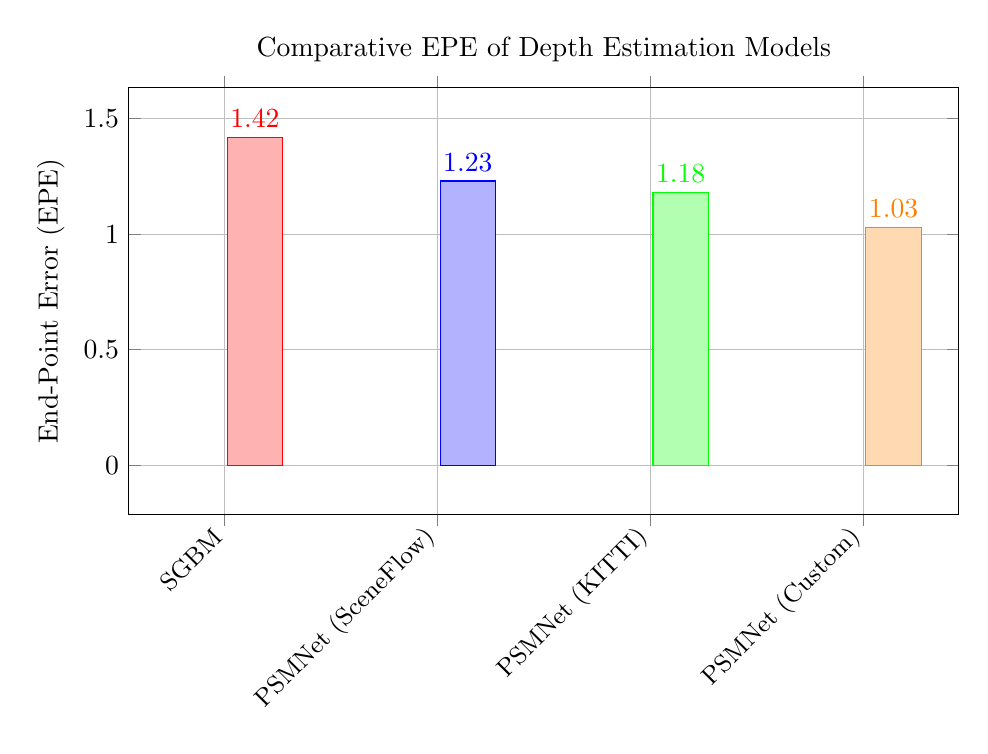
\begin{tikzpicture}
\begin{axis}[
ybar,
enlargelimits=0.15,
ylabel={End-Point Error (EPE)},
symbolic x coords={SGBM, PSMNet (SceneFlow), PSMNet (KITTI), PSMNet (Custom),  },
xtick=data,
nodes near coords,
nodes near coords align={vertical},
x tick label style={rotate=45, anchor=east, font=\small},
ymin=0,
bar width=20pt,
width=\columnwidth,
height=7cm,
grid=major,
legend pos=north east,
title={Comparative EPE of Depth Estimation Models}
]
\addplot[style={red,fill=red!30},forget plot] coordinates {(SGBM, 1.42)};
\addplot[style={blue,fill=blue!30},forget plot] coordinates {(PSMNet (SceneFlow), 1.23)};
\addplot[style={green,fill=green!30},forget plot] coordinates {(PSMNet (KITTI), 1.18)};
\addplot[style={orange,fill=orange!30},forget plot] coordinates {(PSMNet (Custom), 1.03)};
\end{axis}
\end{tikzpicture}
\caption{Comparison of End-Point Error (EPE) for different depth estimation models against the ToF camera ground truth. The custom-trained PSMNet achieves the lowest error.}
\label{fig:epe_comparison}
\end{figure}

Qualitative inspection of the generated 3D point clouds further supports these quantitative findings. The SGBM-derived point cloud (Fig. \ref{fig:sgbm_point_cloud}) exhibits significant noise and sparsity, particularly on uniform surfaces. In contrast, the point cloud from the custom-trained PSMNet (Fig. \ref{fig:psmnet_point_cloud}) is substantially denser and more coherent.

\begin{figure}[htbp]
\centerline{\includegraphics[width=0.7\columnwidth]{sgbm_pointcloud.png}}
\caption{Point Cloud generated from SGBM algorithm.}
\label{fig:sgbm_point_cloud}
\end{figure}

\begin{figure}[htbp]
\centerline{\includegraphics[width=0.7\columnwidth]{psmnet_pointcloud.png}}
\caption{Point clouds generated from the custom-trained PSMNet.}
\label{fig:psmnet_point_cloud}
\end{figure}

The superior performance of the custom-trained PSMNet model underscores the criticality of domain-specific fine-tuning for maximizing depth estimation accuracy. However, this quantitative success is tempered by several challenges. Despite the improvement, visual inspection of the PSMNet point cloud reveals residual artifacts and surface distortions, likely due to the limited size and diversity of our custom training dataset. Furthermore, the system remains sensitive to variations in ambient lighting, a persistent issue for passive vision sensors. These factors collectively indicate that while deep learning significantly enhances stereo vision, achieving LiDAR-grade reliability requires more extensive training data and robust solutions for environmental variability \cite{yao2025stereo}. The current system can approximate LiDAR-level mapping, but its effectiveness is highly contingent on precise calibration and controlled conditions.

% \section{Methodology}
% This section details the experimental setup and the systematic approach taken to achieve deep learning-enhanced stereo vision for LiDAR emulation in precise robotic arm manipulation.

% \subsection{Hardware Setup}
% The hardware configuration was designed to facilitate robust depth information capture and precise robotic arm manipulation. The selection of components aimed to balance performance with cost-effectiveness, a primary motivation of this research.

% \subsubsection{Robotic Arm}
% A custom-built four-degree-of-freedom (4-DOF) robotic arm was constructed to serve as the manipulation platform. The arm was fabricated using 3D-printed Polylactic acid (PLA) filament for critical joints and custom parts, and aluminum for primary arm segments requiring higher strength and rigidity.

% For actuation, the robotic arm employs NEMA 17 stepper motors with TMC2208 drivers for precision and silent operation. Limit switches ensure accurate position control. A geared mechanism, incorporating herringbone gears, enhances torque and minimizes backlash for smooth, accurate motion.

% The control system consists of an Arduino Uno microcontroller paired with an Arduino CNC shield, providing sufficient I/O and processing power for real-time control. A 30A Switch Mode Power Supply (SMPS) ensures consistent voltage delivery. The choice of 3D-printed components and an Arduino-based control system reflects a deliberate strategy for cost-effective prototyping.

% \begin{figure}[htbp]
% \centerline{\includegraphics[width=0.7\columnwidth]{robotic_arm.jpg}}
% \caption{Custom-built 4-DOF robotic arm.}
% \label{fig:robotic_arm}
% \end{figure}

% \subsubsection{ToF and Stereo Camera System}
% The integration of Time-of-Flight (ToF) and stereo cameras is fundamental for capturing comprehensive depth information. The ToF camera, specifically the MaixSense-A075V, serves as the ground truth source for precise depth data \cite{hansard2012time}. Its specifications are:
% \begin{itemize}
%     \item \textbf{Depth Resolution}: 320x240 at 60 frames per second.
%     \item \textbf{Field of View}: 55° (Horizontal) x 72° (Vertical).
%     \item \textbf{Operating Range}: 0.15 to 1.5 meters.
%     \item \textbf{Connection}: USB 2.0 Type-C.
%     \item \textbf{Additional Features}: RGB resolution of 1600x1200 at 30 fps, RGB field of view of 120°.
% \end{itemize}
% For stereo vision, two Fantech Luminous C30 cameras were employed. Their specifications include:
% \begin{itemize}
%     \item \textbf{Resolution}: 2560x1440 at 25 frames per second.
%     \item \textbf{Field of View}: 106°.
%     \item \textbf{Connection}: USB 2.0.
%     \item \textbf{Dimensions}: 73 x 26 x 33 mm.
%     \item \textbf{Weight}: 87 grams.
% \end{itemize}
%  The precise measurements provided by the ToF camera are essential for serving as the ground truth reference during DNN training.

% \begin{figure}[htbp]
% \centerline{\includegraphics[width=\columnwidth]{camera_setup.png}}
% \caption{ToF and Stereo Camera System.}
% \label{fig:cameras}
% \end{figure}

% \subsubsection{Workspace Setup}
% The workspace was designed to facilitate efficient and controlled data collection and testing. It consists of a sturdy wooden frame supporting the setup, with a flat, rigid base platform for mounting the robotic arm and objects.

% Both the stereo camera rig and the ToF camera are mounted at the top of the frame, allowing for a wide, overlapping view of the workspace. A laptop controls the robotic arm via serial communication and collects real-time camera data. Consistent, well-lit conditions are maintained to optimize camera performance.

% \begin{figure}[htbp]
% \centerline{\includegraphics[width=0.7\columnwidth]{workspace_setup.jpg}}
% \caption{Workspace setup for data acquisition and robotic arm operation.}
% \label{fig:workspace}
% \end{figure}

% \subsection{Camera Calibration}
% Camera calibration is a foundational step in any vision-based system, ensuring the geometric accuracy necessary for reliable 3D reconstruction and depth estimation \cite{liao2303deep}.

% \subsubsection{Importance of Calibration}
% Camera calibration estimates intrinsic and extrinsic parameters to accurately map 3D points to 2D projections. This process is paramount for:
% \begin{itemize}
%     \item \textbf{Correcting Lens Distortions}: Real-world lenses introduce distortions (radial, tangential) that must be corrected for accurate image representation.
%     \item \textbf{Accurate Depth Estimation}: Calibration ensures precise alignment of stereo cameras, critical for accurate disparity map computation and depth inference.
%     \item \textbf{Reliable 3D Reconstruction}: By accurately mapping 2D image points to 3D world coordinates, calibration facilitates reliable 3D reconstruction, essential for precise spatial understanding.
% \end{itemize}

% \subsubsection{Epipolar Geometry}
% Epipolar geometry describes the geometric relationship between two camera views of the same 3D scene \cite{xu2013epipolar, hartley2003multiple}. It is defined by a 3D point and the optical centers of the two cameras, forming the epipolar plane. The intersection of this plane with the image planes creates epipolar lines, which constrain the possible locations of corresponding points, significantly reducing the search space. When image planes are parallel, epipolar lines align horizontally, simplifying correspondence.

% The camera's intrinsic matrix $\mathbf{K}$ defines its internal optical properties:
% $$\mathbf{K} = \begin{pmatrix} f_x & 0 & c_x \\ 0 & f_y & c_y \\ 0 & 0 & 1 \end{pmatrix} \quad (1)$$
% where $f_x$ and $f_y$ are focal lengths, and $c_x$ and $c_y$ are optical center coordinates. Extrinsic parameters ($\mathbf{R}$, $\mathbf{t}$) describe orientation and position relative to a world coordinate system:
% $$\mathbf{X}_c = \mathbf{R}\mathbf{X}_w + \mathbf{t} \quad (2)$$
% Lens distortions are corrected using radial ($K_1, K_2, K_3$) and tangential ($P_1, P_2$) coefficients. Corrected image coordinates ($x'', y''$) from distorted coordinates ($x', y'$) are given by:
% $$x'' = x'(1+K_1r^2+K_2r^4+K_3r^6)+2P_1x'y'+P_2(r^2+2x'^2) \quad (3)$$
% $$y'' = y'(1+K_1r^2+K_2r^4+K_3r^6)+P_1(r^2+2y'^2)+2P_2x'y' \quad (4)$$
% where $r^2=x'^2+y'^2$.

% \subsubsection{Challenges in Hardware Alignment and Stereo Rectification as Solution}
% Achieving perfectly parallel image planes through hardware alignment is challenging due to intricate mounting mechanisms, lens imperfections, and environmental factors. Even minor misalignments or distortions can lead to substantial errors in depth estimation.

% Stereo rectification serves as the crucial software-based solution \cite{zhao2024dive, gong2025rectification}. This process geometrically transforms images so that epipolar lines become parallel and horizontal, simulating the ideal parallel configuration. This ensures corresponding points are aligned horizontally, significantly facilitating accurate disparity calculation and subsequent depth estimation.

% \subsubsection{Calibration Process}
% The calibration process involved capturing multiple images of a checkerboard pattern (9x7) from various angles and distances \cite{zhang2002flexible, zhang1999flexible}. Corners were detected using OpenCV's \texttt{findChessboardCorners} algorithm. Subsequently, the \texttt{calibrateCamera} function estimated the intrinsic and extrinsic parameters by analyzing the relationship between 2D image points and their known 3D positions.

% \subsubsection{Parameters Derived from Calibration}
% The intrinsic parameters and distortion coefficients for the Fantech Luminous C30 cameras were precisely determined. These parameters are crucial for accurate 3D reconstruction and precise mapping of 3D world points to 2D image projections. The determined parameters are listed in Table \ref{tab1}.

% \begin{table}[htbp]
% \caption{Fantech Luminous C30 Camera Intrinsic Parameters and Distortion Coefficients}
% \begin{center}
% \begin{tabular}{|c|c|}
% \hline
% \textbf{Parameter}&\textbf{Value} \\
% \hline
% $f_x$ & 680.9335952 mm \\
% $f_y$ & 681.53275369 mm \\
% $c_x$ & 322.60859724 px \\
% $c_y$ & 257.99884455 px \\
% $K_1$ & -3.84198386 $\times$ 10$^{-1}$ \\
% $K_2$ & 3.37282195 $\times$ 10$^{-1}$ \\
% $K_3$ & 1.72120651 $\times$ 10$^{-3}$ \\
% $P_1$ & -5.48946011 $\times$ 10$^{-4}$ \\
% $P_2$ & -6.45215020 $\times$ 10$^{-1}$ \\
% \hline
% \end{tabular}
% \label{tab1}
% \end{center}
% \end{table}

% \subsubsection{Calibration Results}
% The camera calibration process significantly improved image quality and geometric accuracy. In the undistorted image, the checkerboard pattern displayed perfectly straight lines, indicating successful correction of lens distortions. The Root Mean Square (RMS) error for the rectification process was 1.50921, well below the acceptable threshold of 2, confirming successful epipolar alignment for subsequent disparity map generation.
% `
% \begin{figure}[htbp]
% \centerline{\includegraphics[width=\columnwidth]{rectified_camera_view.png}}
% \caption{Rectified camera view demonstrating epipolar alignment.}
% \label{fig:rectification}
% \end{figure}

% \subsection{Data Acquisition}
% Data acquisition is a critical phase, involving capturing data to train and validate depth estimation algorithms. The data collection involved capturing images and depth maps across various scenes and lighting conditions, including diverse textures, shapes, and distances. The ToF camera captured depth maps, $D(x, y)$, where each pixel represents distance. Simultaneously, stereo cameras captured image pairs, $I_L(x, y)$ and $I_R(x, y)$, used to compute disparity maps. The disparity $d(x, y)$ is the horizontal shift between corresponding points:
% $$d(x, y) = x_L - x_R \quad (5)$$
% where $x_L$ and $x_R$ are x-coordinates of corresponding points. Depth $Z$ is estimated using triangulation:
% $$Z = \frac{f \cdot B}{d(x,y)} \quad (6)$$
% where $f$ is focal length, and $B$ is the baseline distance (84.85mm in this setup).

% \subsection{Depth Estimation (Traditional SGBM)}
% This section details the initial depth estimation using a traditional stereo matching algorithm, establishing a baseline for subsequent deep learning enhancements.

% \subsubsection{Theoretical Framework}
% The fundamental principle of stereo depth estimation relies on triangulation between corresponding points in rectified image pairs. Utilizing the calibrated stereo setup with a precisely measured baseline distance of 84.85mm, depth computation adheres to the established relationship presented in Equation (6).

% \subsubsection{Implementation Architecture (Semi-Global Block Matching - SGBM)}
% The Semi-Global Block Matching (SGBM) algorithm was implemented for initial disparity map generation \cite{hirschmuller2007stereo, hernandez2016embedded}. SGBM was chosen for its superior performance in maintaining both global consistency and local detail preservation, offering a robust balance between accuracy and computational efficiency. The optimized parameter configuration for the specific indoor robotics use case is detailed in Table \ref{tab2}.

% \begin{table}[htbp]
% \caption{SGBM Algorithm Optimized Parameters}
% \begin{center}
% \begin{tabular}{|c|c|c|}
% \hline
% \textbf{Parameter} & \textbf{Value}  \\
% \hline
% Block Size & 7 pixels  \\
% Disparity Range & 128 levels \\
% Minimum Disparity & 5  \\
% P1 Penalty & 8 * 3 * 7$^2$  \\
% P2 Penalty & 32 * 3 * 7$^2$  \\
% Uniqueness Ratio & 15  \\
% Speckle Window Size & 100  \\
% Speckle Range & 2  \\
% Pre-Filter Cap & 63 \\
% \hline
% \end{tabular}
% \label{tab2}
% \end{center}
% \end{table}

% \begin{figure}[htbp]
% \centerline{\includegraphics[width=\columnwidth]{sgbm_depth_and_disparity.png}}
% \caption{Depth map and Disparity map generated using the SGBM algorithm.}
% \label{fig:sgbm_depth}
% \end{figure}

% \subsubsection{Results Analysis}
% The SGBM-based depth estimation system demonstrated an effective depth range of 100mm to 2000mm, suitable for indoor robotics. It maintained high spatial resolution, distinguishing foreground and background objects while preserving surface continuity. Quality was evident in well-textured regions with minimal noise. Edge detection at depth discontinuities remained sharp and accurate. Visual verification consistently showed appropriate depth gradients. However, in low-textured regions, the system occasionally produced noisy depth estimates, slightly degrading performance in such areas.

% % ===================================================================
% % DEEP LEARNING ENHANCEMENT SECTION
% % ===================================================================
% \subsection{Deep Learning Enhancement (PSMNet)}
% To overcome the inherent limitations of traditional stereo matching algorithms, a deep learning-based approach was implemented to refine depth estimation.

% \subsubsection{Challenges of Traditional Methods}
% Traditional algorithms like SGBM are known to suffer from matching ambiguities in textureless or uniformly textured regions, resulting in inaccurate or noisy depth maps that are unreliable for precise robotic tasks.

% \subsubsection{PSMNet Architecture}
% To address these challenges, the Pyramid Stereo Matching Network (PSMNet) architecture was employed \cite{chang2018pyramid}. PSMNet is effective at resolving ambiguities by leveraging global contextual information through three primary components: a CNN-based \textit{Feature Extraction Module}, a multi-scale \textit{Spatial Pyramid Pooling (SPP)} module, and a \textit{3D Stacked Hourglass Module} for cost volume regularization and disparity regression.

% \begin{figure}[htbp]
% \centerline{\includegraphics[width=\columnwidth]{psmnet_architecture.png}}
% \caption{Simplified architecture of the PSMNet \cite{chang2018pyramid}}
% \label{fig:psmnet_architecture}
% \end{figure}

% \subsubsection{Comparative Evaluation and Custom Training}
% A comparative evaluation was conducted to quantify the performance gains from deep learning. The End-Point Error (EPE) metric was used to evaluate the following models against ground truth data from the ToF camera:
% \begin{itemize}
%     \item \textbf{SGBM Algorithm}: The traditional baseline.
%     \item \textbf{Pre-trained PSMNet (SceneFlow)}: A model trained on a large-scale synthetic dataset.
%     \item \textbf{Pre-trained PSMNet (KITTI)}: A model trained on a real-world autonomous driving dataset.
%     \item \textbf{Custom-Trained PSMNet}: A model fine-tuned for 1500 epochs on a custom-captured dataset from the experimental setup.
% \end{itemize}

% \subsubsection{Results and Analysis}
% The evaluation results are summarized in Figure \ref{fig:epe_comparison}. The baseline SGBM algorithm yielded an EPE of 1.42. Pre-trained PSMNet models demonstrated improved performance, with the KITTI-trained model reaching an EPE of 1.18. The custom-trained PSMNet achieved the lowest error (EPE=1.03), a 27\% improvement over the SGBM baseline. This highlights the significant benefit of domain-specific fine-tuning. Despite the quantitative improvement, visual inspection of the resulting point clouds (Figures \ref{fig:sgbm_point_cloud} and \ref{fig:psmnet_point_cloud}) revealed residual artifacts, likely due to the limited size of the training dataset.

% \begin{figure}[htbp]
% \centering
% \begin{tikzpicture}
% \begin{axis}[
% ybar,
% enlargelimits=0.15,
% ylabel={End-Point Error (EPE)},
% symbolic x coords={SGBM, PSMNet (SceneFlow), PSMNet (KITTI), PSMNet (Custom),  },
% xtick=data,
% nodes near coords,
% nodes near coords align={vertical},
% x tick label style={rotate=45, anchor=east, font=\small},
% ymin=0,
% bar width=20pt,
% width=\columnwidth,
% height=7cm,
% grid=major,
% legend pos=upper right,
% title={Comparative EPE of Depth Estimation Models}
% ]
% \addplot[style={red,fill=red!30},forget plot] coordinates {
% (SGBM, 1.42)
% };
% \addplot[style={blue,fill=blue!30},forget plot] coordinates {
% (PSMNet (SceneFlow), 1.23)
% };
% \addplot[style={green,fill=green!30},forget plot] coordinates {
% (PSMNet (KITTI), 1.18)
% };
% \addplot[style={orange,fill=orange!30},forget plot] coordinates {
% (PSMNet (Custom), 1.03)
% };

% % \addlegendimage{blue,fill=blue!30}
% % \addlegendentry{EPE vs. ToF Ground Truth}
% \end{axis}
% \end{tikzpicture}
% \caption{Comparison of End-Point Error (EPE) for different depth estimation models against the ToF camera ground truth. The chart shows a clear performance hierarchy, with the custom-trained PSMNet achieving the lowest error.}
% \label{fig:epe_comparison}
% \end{figure}

% \begin{figure}[htbp]
% \centerline{\includegraphics[width=0.7\columnwidth]{sgbm_pointcloud.png}}
% \caption{Point Cloud generated from SGBM algorithm.}
% \label{fig:sgbm_point_cloud}
% \end{figure}

% \begin{figure}[htbp]
% \centerline{\includegraphics[width=0.7\columnwidth]{psmnet_pointcloud.png}}
% \caption{Point clouds generated from the custom-trained PSMNet.}
% \label{fig:psmnet_point_cloud}
% \end{figure}

% % ===================================================================
% % RESULTS AND DISCUSSION SECTION
% % ===================================================================
% \section{Results and Discussion}
% The experimental results confirm a clear performance hierarchy, with the custom-trained PSMNet model (EPE=1.03) substantially outperforming both the traditional SGBM baseline (EPE=1.42) and pre-trained networks. This finding underscores the criticality of domain-specific fine-tuning for maximizing depth estimation accuracy.

% However, this quantitative success is tempered by several challenges. The model's generalization was constrained by the limited size and diversity of our custom training dataset. Furthermore, the system remained sensitive to variations in ambient lighting, a persistent issue for passive vision sensors. Finally, the computational overhead of training deep neural networks remains a practical consideration.


% These factors collectively indicate that while deep learning significantly enhances stereo vision, achieving LiDAR-grade reliability requires more extensive training data and robust solutions for environmental variability \cite{yao2025stereo}. The current system can approximate LiDAR-level mapping, but its effectiveness is highly contingent on precise calibration and controlled conditions.

% ===================================================================
% CONCLUSION SECTION
% ===================================================================
% \section{Conclusion}
% This research investigated the efficacy of deep learning-enhanced stereo vision as a cost-effective alternative to LiDAR for robotic manipulation. A comparative analysis demonstrated that a custom-trained Pyramid Stereo Matching Network (PSMNet) model significantly reduces depth estimation error in contrast to a conventional SGBM algorithm and pre-trained networks. The results confirm that domain-specific fine-tuning is crucial for maximizing performance. However, challenges related to limited training data and environmental sensitivity prevent the system from achieving full LiDAR-comparable reliability. The findings validate the potential of this approach but highlight that its effectiveness is contingent on domain-specific training and controlled operating conditions.

\section{Conclusion}
This research successfully demonstrated the potential of deep learning-enhanced stereo vision as a cost-effective alternative to LiDAR for high-precision robotic manipulation. Our principal finding is that a Pyramid Stereo Matching Network (PSMNet) fine-tuned on a domain-specific dataset significantly outperforms both traditional algorithms and pre-trained deep learning models. This custom-trained network achieved a 27\% reduction in End-Point Error compared to the SGBM baseline, as well as a notable improvement over networks pre-trained on generic autonomous driving and synthetic datasets. This result underscores the critical impact of mitigating domain shift; while pre-trained models offer a strong foundation, adapting them to the specific sensor characteristics, lighting conditions, and object distributions of the target workspace is paramount for maximizing accuracy.

Consequently, our work validates this approach as a viable pathway toward affordable, high-fidelity 3D perception in controlled environments. It presents a clear trade-off for system designers: for applications where environmental conditions can be regulated, this method offers LiDAR-approximate performance at a fraction of the cost. Nevertheless, the system's performance remains contingent on the quality and scope of training data and is susceptible to ambient lighting variations, indicating that it has not yet achieved the all-conditions robustness of active sensors.

\section{Future Work}
Building upon this work, our primary future direction is to enhance system robustness by addressing the current data limitations. We plan to create a larger and more diverse training dataset by integrating higher-fidelity sensors, such as a commercial LiDAR unit or an Intel RealSense camera. This will provide more precise ground-truth data and enable the model to generalize better across a wider range of objects and scenarios.

Second, to rigorously validate the practical utility of the enhanced depth maps, the current 4-DOF manipulator will be upgraded to a more rigid, industrial-grade 6-DOF platform. Incorporating force-torque sensing at the wrist will allow for quantitative evaluation of closed-loop manipulation tasks, such as peg-in-hole insertion or grasping objects with arbitrary poses, thereby directly correlating depth map accuracy with task success.

Further research will extend the system's application to dynamic environments. This involves investigating methods for real-time performance optimization and exploring multi-sensor fusion techniques that synergistically combine the dense, textured output of stereo vision with sparse but highly accurate data from other modalities. The goal is to create a perception system that is robust to environmental changes and moving objects. Finally, we will explore more advanced deep learning architectures, such as vision transformers or hybrid CNN-transformer models, which may offer improved handling of global context and long-range dependencies, potentially yielding further improvements in depth estimation accuracy and reducing artifacts in textureless regions.

% \bibliographystyle{plain} 
% \bibliography{references}

\bibliographystyle{IEEEtran} 
\bibliography{references}
\end{document}
